\section{Chap1-CommunicationBasics}
\subsection*{NETWORKING BASICS}
ISO OSI: Open Systems Interconnection model, Basis for standards development on systems interconnection.
% TODO: wait to be added
\subsection*{SOCKET}
Move data/message/(invoke operation/service and return result/failure) from Application I on Host A to Application K on Host B.
\rtext{Client}:Issues requests to server(send \& receive).
\rtext{Server}:Starts up and listens for connections, requests, and sends/receives.
\rtext{Client/Server examples}: telnet/telnetd, ftp/ftpd (sftp/sftpd), Firefox/Apache.
\rtext{Socket}: network programming abstraction for communicating among processes (applications) based on (Unix) file
descriptors.
\rtext{File descriptor}:an integer representing an open file managed by the OS \textbackslash In Unix any I/O is done by reading/writing from/to file
descriptors.
\rtext{Socket types}: 
Stream socket:java.net.ServerSocket, TCP based, Ordering guaranteed, Error-free 
\textbackslash Datagram socket:java.net.DatagramSocket, UDP based 
\textbackslash IPv4 \& IPv6

% TODO: add this pic surrowed by words
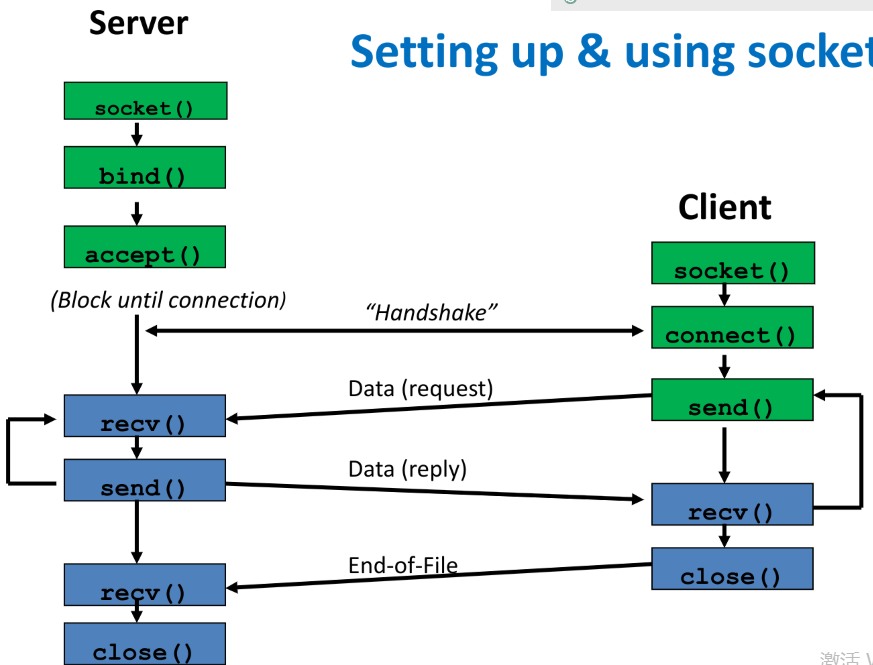
\includegraphics[width=.8\linewidth]{chap1_1.png}
\subsection*{NIO(Nonblocking sockets)}
\rtext{Synchronous}: Single thread reading data from clients(stream) and blocked until ready(no multiple read)
\rtext{Asynchronous}: Single thread reading data from clients: Thread $\rightarrow$ Channel: read data into buffer, Channel $\rightarrow$ Buffer: fill data into buffer, Thread $\rightarrow$ Buffer: check data in buffer (main thread not blocked)
\rtext{Synchronous vs. Asynchronous}: 
S: A thread enters into action and waits until I/O is completed \textbackslash Limited scalability, one thread per I/O connection(Overhead:context switching $\rightarrow$ time between diff. tasks)
A: Passes the request immediatly to the OS-kernel and then do other tasks $\rightarrow$ worker thread \lstinline{while(true){} only do computation, never blocked, no context swtich
\rtext{Java NIO Channels}: All IO operations can be done with channels(File, TCP, UDP) 
\textbackslash Multiple types of channels(FileChannel (File on disk),DatagramChannel (UDP), SocketChannel (TCP, support concurrent read/write), ServerSocketChannel (TCP))
\textbackslash Responsibilities(Read, write buffer)

\rtext{U1}
Finite state machines that describe \rtext{a communication session between a client and a server}.
The first FSM represents the server and the second FSM represents the client. Both parties (client and server) keep the communication session open and exchange messages until one of them decides to close it
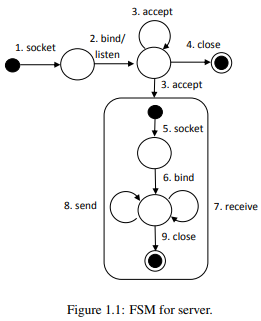
\includegraphics[width=.45\linewidth]{chap1_2.png} 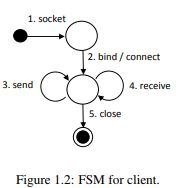
\includegraphics[width=.45\linewidth]{chap1_3.png}
$accept$ is \lstinline{while loop}, detail in rectangle: create a new socket (and therad) for commu. with client
\rtext{Simple protocol design}  complex number as string: $c_i = (a, b)$, $op \in \{add, sub, mul, div\}$,
C to S message format: $m_1 \textless c_1;c_2;op \textgreater$,
Status: $st \in \{ OK,msgIncomplete, ... \}$,
S to C message format: $m_2 \textless C_r; st \textgreater$
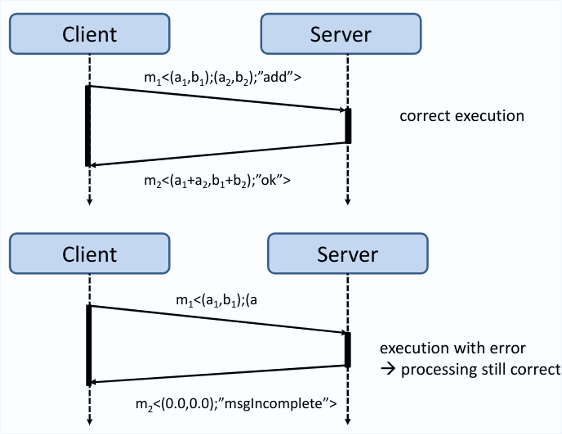
\includegraphics[width=.45\linewidth]{chap1_4.png} 

% TODO: code about socket clien server